\newcommand{\rmse}[1]{
	\vspace*{-2mm}
	\begin{center}
		\begin{tcolorbox}[colback=white, colframe=iwiPurple, halign=flush center, width=0.8\linewidth, boxrule=1pt, arc=4mm]
				\Acrshort{rmse} :\ \ \textbf{\texttt{#1}}
		\end{tcolorbox}
	\end{center}
}

%%%%%%%%%%%%%%%%%%%%%%%%%%%%%%%%%%%%%%%%%%%%%%%%%%%%%%%%%%%%%%%%%%

After creating a variety of different features, we are now going to apply them on different types of models and compare their performance. To best compare the results, a common metric has been chosen, in particular the one to match the Kaggle competitions evaluation method: \acrfull{rmse}.

%%%%%%%%%%%%%%%%%%%%%%%%%%%%%%%%%%%%%%%%%%%%%%%%%%%%%%%%%%%%%%%%%%
\subsection{Linear Regression}
%%%%%%%%%%%%%%%%%%%%%%%%%%%%%%%%%%%%%%%%%%%%%%%%%%%%%%%%%%%%%%%%%%

In this section we are incrementaly going over the various parameters and inputs applied to the model and examine their direct impact. All steps have been documented in separate GIT commits and linked to the respective commit for reference.

%%%%%%%%%%%%%%%%%%%%%%%%%%%%%%%%%%%%%%%%%%%%%%%%%%%%%%%%%%%%%%%%%%
\subsubsection{Raw data - \commitCompareModels{5df6ba024166903c829daa9c51c5fafa13e2480a}}

To start off, we determined a base score to proceed from. We simply took the train data as it is given at the start of the competition and applied a basic \texttt{LinearRegression}\footnote{\href{https://scikit-learn.org/stable/modules/generated/sklearn.linear_model.LinearRegression.html\#sklearn.linear_model.LinearRegression}{Link to scikit-learn documentation}} from \gls{scikit} on the data.
\rmse{8.10506}


%%%%%%%%%%%%%%%%%%%%%%%%%%%%%%%%%%%%%%%%%%%%%%%%%%%%%%%%%%%%%%%%%%
\subsubsection{Clip raw data - \commitCompareModels{e8b67dc4e6f6813df2d293bd5855879723940d16}}

Now, after carefully reading the \href{https://www.kaggle.com/c/competitive-data-science-predict-future-sales/overview/evaluation}{competitions description}, we found out that the values are intended to be clipped to the $[0;20]$ range. After clipping the train values and reapplying them onto the very same input data, the score increased significantly.
\rmse{2.56222}

%%%%%%%%%%%%%%%%%%%%%%%%%%%%%%%%%%%%%%%%%%%%%%%%%%%%%%%%%%%%%%%%%%
\subsubsection{Add zero sales - \commitCompareModels{ccfe1162ca359dd7ca99b8accc525b053ec8df0d}}

In this step, we have added the zero sales, referenced in section \ref{zerosales}, onto the training data. We can again see a significant increase in the models performance.
\rmse{1.22789}


%%%%%%%%%%%%%%%%%%%%%%%%%%%%%%%%%%%%%%%%%%%%%%%%%%%%%%%%%%%%%%%%%%
\subsubsection{Add feature engineering - \commitCompareModels{1de63b67a09f39dbf74f6c9ba82203149dd339b9}}

Finally, the --- long anticipated --- feature engineered data. How will the model perform now? We can now observe the last significant leap in performance.
\rmse{0.80112}

%%%%%%%%%%%%%%%%%%%%%%%%%%%%%%%%%%%%%%%%%%%%%%%%%%%%%%%%%%%%%%%%%%
\subsubsection{Applying \texttt{cross\_val\_score} - \commitCompareModels{0c0ddf6b624009a9d8740c769a8ec1cecfe8d2a3}}

In order to get a more realistic approximation of the final score on the test data, we have now switched to the more sophisticated \texttt{cross\_val\_score}\footnote{\href{https://scikit-learn.org/stable/modules/generated/sklearn.model_selection.cross_val_score.html}{\texttt{cross\_val\_score} documentation}} evaluation. This action is significantly heavier on execution time, as the same input data is split into various validation sets internally (5 by default).
Unsurprisingly, the performance took a small dent at first.
\rmse{0.82563}

%%%%%%%%%%%%%%%%%%%%%%%%%%%%%%%%%%%%%%%%%%%%%%%%%%%%%%%%%%%%%%%%%%
\subsubsection{Dropping superfluous shops - \commitCompareModels{c47eb457417a0eb117c042227917edf2d913dc6a}}

As observed in the \Acrshort{eda}, about 30\% of the shops present in the train data, are irrelevant to the final test data. In theory, this should not change anything when performing a split on the train data. But, maybe the authors of the competition had certain irregularities, such as the detected price outliers in section \ref{outliers} which is irrelevant for the test prediction, in mind when setting the environment for the competition. Our result was satisfying:
\rmse{0.81432}

%%%%%%%%%%%%%%%%%%%%%%%%%%%%%%%%%%%%%%%%%%%%%%%%%%%%%%%%%%%%%%%%%%
\subsubsection{Applying LASSO regression - \commitCompareModels{b89f6dacc0c95a63d1b2b6da1d09524549eb33b6}}

Next up, we attempted to apply the data to a \acrshort{lasso} model. The result was very shocking: the performance worsen significantly.
\rmse{0.98846}

%%%%%%%%%%%%%%%%%%%%%%%%%%%%%%%%%%%%%%%%%%%%%%%%%%%%%%%%%%%%%%%%%%
\subsubsection{Applying Ridge regression - \commitCompareModels{956c34719afb18c1ecacb1bdfe13656f5b3a6888}}

Now, onto the Ridge model. We were now back to our original performance:
\rmse{0.81432}


%%%%%%%%%%%%%%%%%%%%%%%%%%%%%%%%%%%%%%%%%%%%%%%%%%%%%%%%%%%%%%%%%%
\subsubsection{Applying Ridge cross-validation - \commitCompareModels{a315c8fcf004c256a87f43bf44b9555b66233b80}}

As a final evaluation of different regularization attemps, we tried a cross-validation to determine the best parameters. To our surprise, this did not yield any improvement either:
\rmse{0.81432}

%%%%%%%%%%%%%%%%%%%%%%%%%%%%%%%%%%%%%%%%%%%%%%%%%%%%%%%%%%%%%%%%%%
\subsubsection{Scaling the data - \commitCompareModels{a8ee348f96b5c94eeadda6d4f101f7eff5d17302}}

To finish the comparisons, we examined the effects of applying a scaler to the data prior to the model training. This did not have any significant impact on the performance.
\rmse{0.81148}


%%%%%%%%%%%%%%%%%%%%%%%%%%%%%%%%%%%%%%%%%%%%%%%%%%%%%%%%%%%%%%%%%%
\subsection{ARIMA}
%%%%%%%%%%%%%%%%%%%%%%%%%%%%%%%%%%%%%%%%%%%%%%%%%%%%%%%%%%%%%%%%%%

Part of this project was to understand the handling of a forecasting model for a time series. 
For this, the \acrfull{arima} model was used. The \acrshort{arima} acronym is divided into three parts: \cite{MultivariateStatisticsARIMA}

\begin{itemize}
	\vspace*{-3mm}
	\item Autoregressive\\
	Describes the dependency among successive observations.
	\vspace*{-3mm}
	\item Integrated\\
	Amount of differenciations needed to make a nonstationary time series stationary.
	\vspace*{-3mm}
	\item Moving Average\\
	Describes the persistence of a random shock from one observation to the next.
\end{itemize}

With \acrshort{arima} being intended to be used for univariate problems \cite{Gron2017HandsOnML}, we had to modify the data a little bit and create our own narrative. Therefore, we analyzed the data and isolated the item, item \texttt{5822}, that had the most sales across the time series.

Similar to the linear regression, we applied the model on the raw data: this gave us a \acrshort{rmse} of \texttt{5.85736}. After analyzing the data and finetuning the \acrshort{arima} parameters, we were able to increase the performance up to \texttt{5.64160}. Very disenchanting compared to the linear regression model. The final forecast looks as following:

\begin{figure}[h]
  \centering
  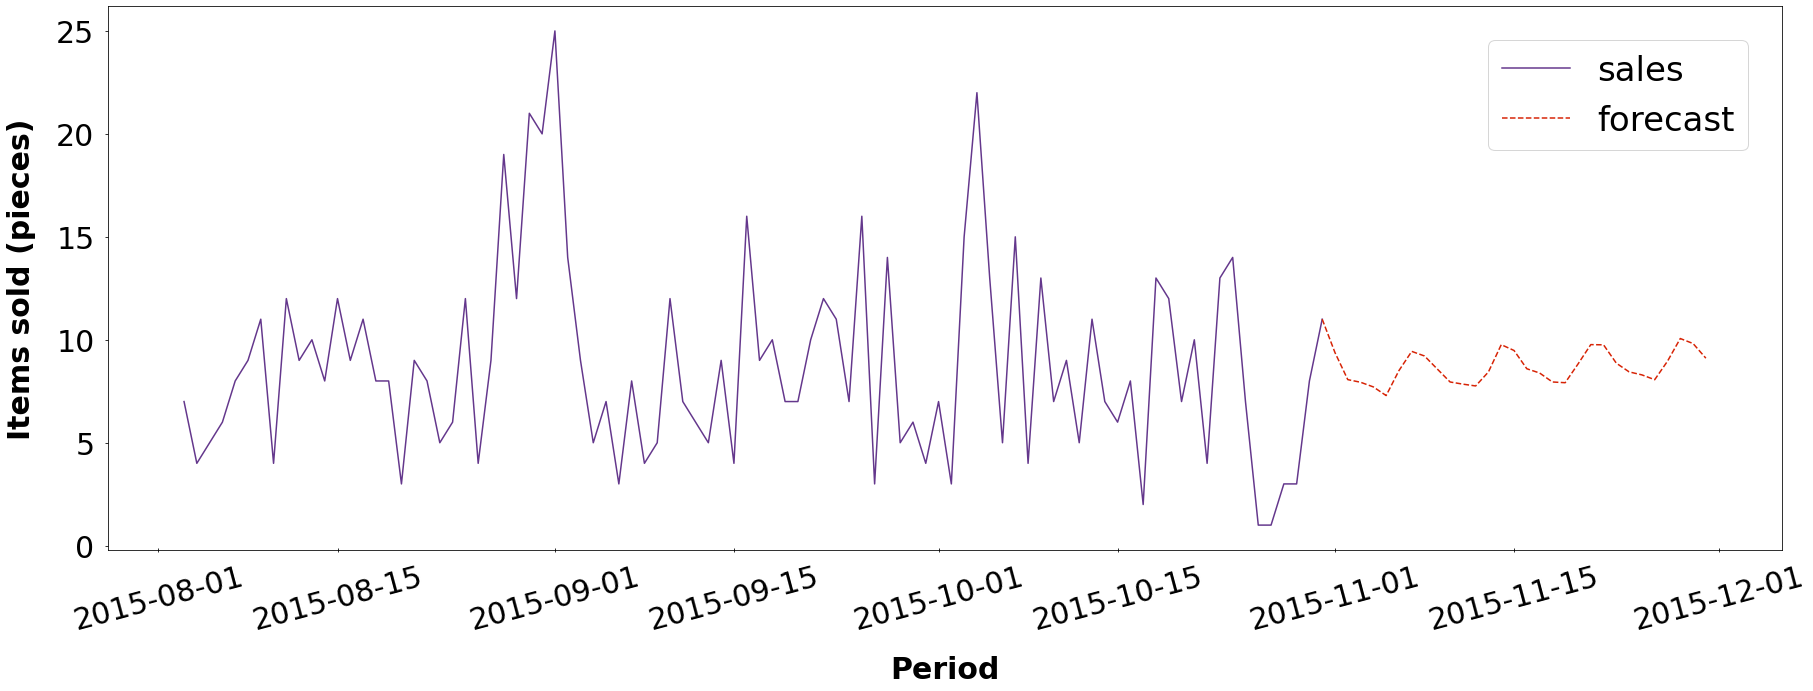
\includegraphics[width=0.88\linewidth]{external_content/graphs/final_arima_forecast.png}
  \captionsetup{justification=centering}
  \captionof{figure}{ARIMA forecast of item \texttt{5822}}
  \label{fig:arima_forecast}
\end{figure}

\vspace*{-8mm}
\begin{center}
\href{\finalARIMAurl}{The step-by-step procedure on how to finetune the \acrshort{arima} parameters can be found here.}
\end{center}
